% !TEX encoding = UTF-8
% !TEX TS-program = pdflatex
% !TEX root = ../tesi.tex

%**************************************************************
\chapter{Integrazione in Route Manager}
\label{cap:integrazione}
%**************************************************************

Le precedenti scelte architetturali, in particolare l'evoluzione per il supporto al concetto di \textit{Context} invece che stato applicativo, sono state dettate dalle esigenze dell'applicazione WorkWave \textit{Route Manager}. 

Tuttavia nonostante ciò l'integrazione ha richiesto anche un significativo lavoro all'interno del codice sorgente dell'applicazione, con aggiunta di logica necessaria puramente per il prodotto in questione per usufruire di \textit{Stargate}. \\

Le modifiche architetturali alla libreria invece sono mirate e portare benefici a tutti i consumatori, non unicamente al prodotto \textit{Route Manager}. \\

Di seguito sono presentate le principali sfide affrontate per l'integrazione.

\section{Google Maps}

L'aspetto più doloroso dell'integrazione è stato Google Maps, tuttavia di vitale importanza per un'applicazione di gestione rotte. Google Maps difatti non è stato progettato per un uso moderno in \textit{Web Workers} e per motivi di compatibilità mantiene comportamenti che lo rendono inadatto all'uso immediato con \textit{Stargate}. \\

Alcune istanze, in particolari della classe \texttt{LatLng} che rappresenta una coordinata geografica, non possiedono campi pubblici ma bensì espongono solo metodi pubblici per poter accedere ai valori di latitudine/longitudine. Tuttavia esse devono essere presenti nello stato applicativo in quanto rappresentano dati fondamentali per l'applicazione e le istanze forniscono i metodi per lavorare agevolmente con tali dati.

Ciò causa però l'impossibilità di trasmetterli dall'applicazione principale verso il \textit{Web Worker} o i widgets, in quanto è impossibile clonare una funzione. L'utilizzo di chiamate RPC §\ref{rpc} è invece proibitivo dato l'estremo alto uso di tali istanze, anche da parte di parti interni di Google Maps ove non è possibile riscrivere il codice affinché gestisca le chiamate RPC asincrone. \\

\subsection{Google Maps serialization}

Il problema ha richiesto di poter configurare la strategia di copia dei dati in \textit{Stargate} durante la trasmissione tra le parti e soprattutto quindi di definirne una propria per Google Maps all'interno di \textit{Route Manager}. In particolare, poiché Google Maps supporta la serializzazione verso il formato \gls{JSON}, è stato obbligatorio serializzare i dati prima della trasmissione di ogni messaggio e ripristinare alla ricezione.

\begin{figure}[H] 
  \centering 
  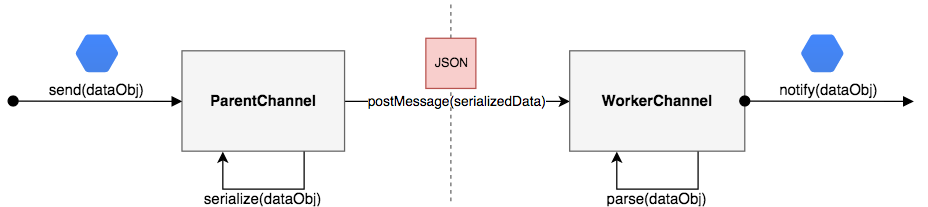
\includegraphics[width=1\columnwidth]{serialization} 
  \caption{Flusso della serializzazione per Google Maps}
\end{figure}

A causa dell'overhead aggiuntivo, vi è stata una particolare attenzione per l'implementazione delle funzioni di serializzazione e parsing, che non puntano a soddisfare tutti i possibili casi d'uso di Google Maps, ma bensì solo quelli in uso nel \textit{Route Manager} con la miglior performance possibile. Il risultato è stato soddisfacente e l'interazione utente con i widgets è fluida. \\

L'utilizzo della serializzazione invece della copia tramite \textit{Structured clone algorithm} ha portato tuttavia ad altri problemi, in particolari quelli descritti come svantaggi di tale strategia alla sezione §\ref{structured-clone}. Ciò ha richiesto del lavoro in più ma non vi è stato nulla di bloccante ed, essendo problemi minori, sono tralasciati da questo documento.

\subsection{Google Maps diffing}

Per motivi analoghi, non è possibile calcolare la differenza tra due oggetti \texttt{LatLng} in quanto hanno solo metodi e non campi dati. In questo caso, l'algoritmo di default per \textit{diff \& patch} è stato esteso in \textit{Route Manager} per supportare tali oggetti. \\

In particolare l'algoritmo normalmente attraversa l'albero dell'oggetto, comparando ogni valore col suo precedente per calcolarne la differenza. In \textit{Route Manager}, tale algoritmo consente di normalizzare i sotto-alberi prima che vengano attraversati per il calcolo e dando quindi la possibilità, nodo per nodo, di rimpiazzare le istanze \texttt{LatLng} con valori che siano comparabili. 

Una volta calcolata la differenza, nell'oggetto \textit{delta} vengono ripristinate le istanze originali di Google Maps ed il delta è pronto per la serializzazione e trasmissione. \\

Poiché la normalizzazione avviene in contemporanea all'attraversamento dell'albero, il costo di performance aggiuntivo è costante in quanto non vi sono maggiori attraversamenti.

\begin{figure}[H] 
  \centering 
  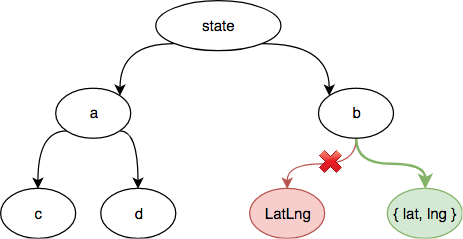
\includegraphics[width=0.75\columnwidth]{normalization} 
  \caption{Esempio di nodo \texttt{LatLng} sostituito con oggetto avente campi comparabili}
\end{figure}

\subsection{ChannelStrategy}

Vista la precedente necessità di poter configurare alcuni aspetti del funzionamento, la libreria \textit{Stargate} fornisce la possibilità di definire un'implementazione dell'interfaccia \texttt{ChannelStrategy}, utilizzata poi internamente per eseguire \textit{diff \& patch} e per sapere il formato dei messaggi. \\

Di seguito si presenta gli aspetti salienti di tale interfaccia, tralasciando alcuni campi minori non menzionati nel documento. \\

\begin{lstlisting}[language={[Sharp]C},basicstyle=\footnotesize]
// Versione semplificata dell'interfaccia
interface ChannelStrategy<TransferFormat> {
  diff: (oldCtx: Context, newCtx: Context) => Delta | undefined
  patch: (ctx: Context, delta: Delta | undefined) => Context

  transfer: (message: Message) => TransferFormat
  receive: (message: TransferFormat) => Message
}
\end{lstlisting}

\texttt{diff/patch} definiscono le funzioni per l'omonimo algoritmo, mentre \texttt{transfer/receive} permettono di trasformare il messaggio dal tipo \texttt{Message} al tipo \texttt{TransferFormat} durante la trasmissione e l'inverso durante la ricezione. \\

La libreria fornisce già due implementazioni di tale interfaccia per un'uso immediato: \texttt{CloneStrategy} basato sullo \textit{Structured clone algorithm} e \texttt{SerializeStrategy} basato sulla serialization. È tuttavia possibile per il consumatore utilizzare una propria implementazione. \\

\texttt{ParentChannel, WorkerChannel} e \texttt{WidgetChannel} sono tutti configurabili con \texttt{ChannelStrategy} e solitamente viene usata la stessa per tutte e tre le classi, ma nulla vieta di usare diversi algoritmi tra le parti. È difatti possibile voler usare un algoritmo \textit{diff \& patch} estremamente ottimizzato per un \texttt{WidgetChannel} sapendone le necessità e limiti.

\begin{figure}[H] 
  \centering 
  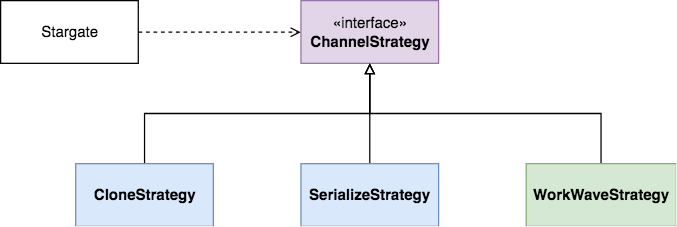
\includegraphics[width=1\columnwidth]{strategy} 
  \caption{Strategy Pattern per la configurazione di Stargate}
\end{figure}
